%%
%% This is file `sample-sigconf.tex',
%% generated with the docstrip utility.
%%
%% The original source files were:
%%
%% samples.dtx  (with options: `sigconf')
%% 
%% IMPORTANT NOTICE:
%% 
%% For the copyright see the source file.
%% 
%% Any modified versions of this file must be renamed
%% with new filenames distinct from sample-sigconf.tex.
%% 
%% For distribution of the original source see the terms
%% for copying and modification in the file samples.dtx.
%% 
%% This generated file may be distributed as long as the
%% original source files, as listed above, are part of the
%% same distribution. (The sources need not necessarily be
%% in the same archive or directory.)
%%
%% Commands for TeXCount
%TC:macro \cite [option:text,text]
%TC:macro \citep [option:text,text]
%TC:macro \citet [option:text,text]
%TC:envir table 0 1
%TC:envir table* 0 1
%TC:envir tabular [ignore] word
%TC:envir displaymath 0 word
%TC:envir math 0 word
%TC:envir comment 0 0
%%
%%
%% The first command in your LaTeX source must be the \documentclass command.

%\documentclass[sigconf]{acmart}
\documentclass[sigconf,screen,nonacm]{acmart}

%% NOTE that a single column version may be required for 
%% submission and peer review. This can be done by changing
%% the \doucmentclass[...]{acmart} in this template to 
%% \documentclass[manuscript,screen]{acmart}
%% 
%% To ensure 100% compatibility, please check the white list of
%% approved LaTeX packages to be used with the Master Article Template at
%% https://www.acm.org/publications/taps/whitelist-of-latex-packages 
%% before creating your document. The white list page provides 
%% information on how to submit additional LaTeX packages for 
%% review and adoption.
%% Fonts used in the template cannot be substituted; margin 
%% adjustments are not allowed.
%%
%%
%% \BibTeX command to typeset BibTeX logo in the docs
\AtBeginDocument{%
  \providecommand\BibTeX{{%
    \normalfont B\kern-0.5em{\scshape i\kern-0.25em b}\kern-0.8em\TeX}}}

%% Rights management information.  This information is sent to you
%% when you complete the rights form.  These commands have SAMPLE
%% values in them; it is your responsibility as an author to replace
%% the commands and values with those provided to you when you
%% complete the rights form.
\setcopyright{acmlicensed}
\copyrightyear{2024}
\acmYear{2024}

%% These commands are for a PROCEEDINGS abstract or paper.
\acmConference[University of Colorado]{CSPB 4502 - Data Mining}{March 18,
  2024}{Boulder, CO}
%
%  Uncomment \acmBooktitle if th title of the proceedings is different
%  from ``Proceedings of ...''!
%
%\acmBooktitle{Woodstock '18: ACM Symposium on Neural Gaze Detection,
%  June 03--05, 2018, Woodstock, NY} 
\acmISBN{978-1-4503-XXXX-X/18/06}


%%
%% Submission ID.
%% Use this when submitting an article to a sponsored event. You'll
%% receive a unique submission ID from the organizers
%% of the event, and this ID should be used as the parameter to this command.
%%\acmSubmissionID{123-A56-BU3}

%%
%% For managing citations, it is recommended to use bibliography
%% files in BibTeX format.
%%
%% You can then either use BibTeX with the ACM-Reference-Format style,
%% or BibLaTeX with the acmnumeric or acmauthoryear sytles, that include
%% support for advanced citation of software artefact from the
%% biblatex-software package, also separately available on CTAN.
%%
%% Look at the sample-*-biblatex.tex files for templates showcasing
%% the biblatex styles.
%%

%%
%% The majority of ACM publications use numbered citations and
%% references.  The command \citestyle{authoryear} switches to the
%% "author year" style.
%%
%% If you are preparing content for an event
%% sponsored by ACM SIGGRAPH, you must use the "author year" style of
%% citations and references.
%% Uncommenting
%% the next command will enable that style.
%%\citestyle{acmauthoryear}

%%
%% end of the preamble, start of the body of the document source.
\begin{document}

%%
%% The "title" command has an optional parameter,
%% allowing the author to define a "short title" to be used in page headers.
\title{COVID-19 Comprehensive Study}

%%
%% The "author" command and its associated commands are used to define
%% the authors and their affiliations.
%% Of note is the shared affiliation of the first two authors, and the
%% "authornote" and "authornotemark" commands
%% used to denote shared contribution to the research.
\author{Mohammed Alsailani}
\authornote{All authors contributed equally to this research.}
\affiliation{%
  \institution{University of Colorado Boulder}
}

\author{Andrew Byrnes}
\authornotemark[1]
\affiliation{%
  \institution{University of Colorado Boulder}
}

\author{Collin Coakley}
\authornotemark[1]
\affiliation{%
  \institution{University of Colorado Boulder}
}


\author{Gilberto Zamarron}
\authornotemark[1]
\affiliation{%
  \institution{University of Colorado Boulder}
}

%%
%% By default, the full list of authors will be used in the page
%% headers. Often, this list is too long, and will overlap
%% other information printed in the page headers. This command allows
%% the author to define a more concise list
%% of authors' names for this purpose.
\renewcommand{\shortauthors}{Alsailani et al. 2024}

%%
%% The abstract is a short summary of the work to be presented in the
%% article.

%%
%% The code below is generated by the tool at http://dl.acm.org/ccs.cfm.
%% Please copy and paste the code instead of the example below.
%%


%%
%% Keywords. The author(s) should pick words that accurately describe
%% the work being presented. Separate the keywords with commas.
%\keywords{COVID-19, Data Mining}

%% A "teaser" image appears between the author and affiliation
%% information and the body of the document, and typically spans the
%% page.


\received{18 Match 2024}
%\received[revised]{18 Match 2024}
%\received[accepted]{18 Match 2024}

%%
%% This command processes the author and affiliation and title
%% information and builds the first part of the formatted document.
\maketitle

\section{Problem Statement/motivation}
Our project focuses on analyzing data related to COVID-19, including the effect of vaccination on transmission, hospitalization, and death. We will also look at other local variables, such as elevation, temperature, humidity, and population density to track the spread of the virus. Our analysis will also use geospatial analysis to look for hot spots and infection surges to see how surrounding counties are impacted. We are relying on the \href{https://health.google.com/covid-19/open-data/}{COVID-19 Open Data by Google}, which provides differing levels of granularity to allow us to focus on different analyses, providing data from 1/1/2020 to 9/17/2022 of various scopes, from world-wide aggregate data, to data about individual counties in any given state in the US. This data was compiled by researchers who authored a paper called \textit{COVID-19 Open-Data a global-scale spatially granular meta-dataset for coronavirus disease} \cite{wahltinez2022covid}.\\ \\
Our motivation is multifaceted. First, COVID-19 is a unique event in our lifetime that impacted the world in an unprecedented way. The urgency of finding a solution to the pandemic resulted in a large amount of data being collected, which makes it a good topic for a data mining project. 
\cite{wahltinez2022covid}. \\

The intriguing questions we aim to answer are:  
\begin{itemize}
    \item How are COVID rates correlated with local variables such as: \begin{enumerate}
        \item Temperature % maybe use a 2 week moving avg of temp & 1-week new COVID cases
        \item Elevation % since elevation is static, we would want to look at cumulative cases
        \item Humidity % maybe 2 week moving avg
        \item Population density %maybe , affect COVID rates? 
        \item Age % Are older individuals more susceptible to mortality?
        \item Sex %Investigating whether sex has any influence on COVID-19 outcomes.
    \end{enumerate}
    \item Classification of counties or general areas COVID-19 hotspots using geospatial analysis
        \begin{enumerate} 
            \item potential classification of areas as hot spots or areas experiencing a surge in infections
            \item The effect of a surge on surrounding areas, including an attempt to analyze factors, such as mobility, that make an area more or less resistant to a surge in cases when nearby area(s) is experiencing a surge.
        \end{enumerate}

    
\end{itemize}
% Interesting questions

%comment block
\begin{comment}
This is a commented-out section using the comment package.
None of the text within the \begin{comment} ... \end{comment} block will be processed by LaTeX.
\end{comment}

\section{Literature survey}
A broad range of prior work has been performed on this data due to significant global impact of COVID-19 on society in the past four years. This data has been applied to economic impact analysis, public health policy analysis, modeling the spread of the virus, assessment of containment measure success and failure, health and healthcare impact forecasts, and more. This dataset has informed researchers, scientists, and healthcare workers in numerous facets of their efforts to effectively allocate resources for vaccine distribution and information dissemination to combat the spread of COVID-19. Fuchs, A. et al \cite{fuchs2020mask} used the dataset to analyse China’s exports of medical goods in times of COVID-19. Arpino, B., et al \cite{arpino2020no} used the data to show that available evidence on the link between intergenerational relationships and COVID-19 is inconclusive. While Murrell, H. et al \cite{murrell2020estimating} used the data to to estimate Rt from Covid-19 data, using SIR models. Studying how infection or vaccination triggers both cellular and humoral responses is essential to know the grade and length of protection generated in the population.

\section{Data set}

The COVID-19 Open Data can be downloaded as world-wide aggregate data, but the data for some countries was sparse in comparison to the US data by county, which was more reliably reported in this dataset. As such, while we plan to clean our data to account for missing values or sparse data, we believe a stronger foundation in the US data by county presents a better baseline dataset for purposes of data mining in this class. As such, we downloaded each US state by county, for a total of 3,228 CSV files with 991 rows of data each on average, and we are storing that in our \href{https://github.com/CCoakley6/DataMiningProjectSpring2024}{group GitHub}. COVID-19 Open Data is most comprehensive COVID-19 dataset we are aware of. It contains collection of epidemiological metrics, including cases, deaths, recoveries, and tests, with variability in data availability across different regions. It highlights the differentiation between new and cumulative data to accommodate adjustments in counting criteria and corrections.

\section{Proposed Work}

\begin{comment}
    - classification: hot spots/zones for mortality, infection, death
    - geographical analysis: (need to pull in geospatial data) of the spread (potentially from areas identified as hot spots or areas that had recent high infection)
    - correlation: between temperature, humidity, etc
\end{comment}

\textbf{Data Transformation}: The data will undergo normalization to incorporate population size, allowing for a more accurate assessment of rates related to high cases, death rates, and vaccination rates. Different normalization methods will be implemented to evaluate their effect on the data such as logarithmic scaling to linearize the data, min-max scaling, population density, and z-score standardization.Below are some considered formulas.
\begin{align*}
\text{Min-Max Scaling:} \quad x_i' &= \frac{{x_i - x_{\text{min}}}}{{x_{\text{max}} - x_{\text{min}}}} \\
\text{Z-score Standardization:} \quad z_i &= \frac{{x_i - \mu}}{{\sigma}} \\
\text{Logarithmic scaling:} \quad x_i' &= \log(x_i) \\
\end{align*}
\\
\textbf{Data Repositories}: Currently we maintain a primary repository for our project at \href{https://github.com/CCoakley6/DataMiningProjectSpring2024}{DataMiningProjectSpring2024}. We have all county CSVs stored for our final product, and we have a subselection of test CSVs to test our data mining functions/strategies before deploying it to the larger dataset.\\
%% Data reduction: get rid of low % columns with few rows, or ones that we don't care to analyze
\\
\textbf{Data Reduction}: The dataset primarily focuses on values relevant to the United States due to the abundance of available data. Furthermore, concerns arise regarding the consistency and reliability of data across different countries due to limitations in resources for tracking cases and deaths. Additionally, the dataset exhibits high dimensionality, prompting the need for a dimension reduction analysis to extract dimensions of interest. Lastly, repeated elements conveying identical information will be consolidated to further diminish the dataset's size.\\
\\
\textbf{Data Cleaning}: Our data will undergo meticulous checks to ensure consistency in data types. While our dataset is fortunate to be rich in quality, we will still thoroughly review it for any inconsistencies or anomalies to maintain its integrity. \\
%% creating a moving avg to track temperature, humidity in relation to new cases (also on a moving avg)
\\
\textbf{Data Aggregation}: The data will be presented in weekly,monthly, and yearly intervals,showcasing the progression of COVID-19 cases, deaths, and vaccination rates. Geographically the data will split into counties or states to see how the virus was handles by each respective group.\\ 
%% geospatial stuff?
\\
\textbf{Data Integration}: The COVID-19 data will be merged with a shapefile depicting the geographical mapping of the United States. This integration aims to provide a territorial representation of how the virus behaves across different regions. \\
\\
\textbf{Regression models}: Linear regression models will be used to help predict transmission rates/mortality rates with regards to a variables such as population density, temperature, humidity, and interventions like vaccination. By fitting a regression line to historical data. \\
\\
\textbf{Logarithmic plot}: Do to the nature of virus growing exponentially a logarithmic plot will linearize the data which may help in trends and growth rates. \\
\\
%% correlation analysis?
\textbf{Scatter plot}: This particular plotting method is useful in identifying correlations among variables. \\
\\
\textbf{Geographical analysis}: We will leverage Geopandas to investigate visual hotspots/zones related to mortality, infection, and fatality. Additionally, we can potentially employ this tool for clustering analysis. \\ 
\\
\textbf{Previous literature}: The profound impact of COVID-19 on the world occurred during an era characterized by widespread access to information, leading to extensive research efforts due to its global significance. As a result, many of the data analysis techniques utilized in our study have already been used to some extents in previous research papers. Despite the similarities in techniques used in previous literature, our dataset appears to have been underutilized in comparison. As a result, there may be differences between our findings and those of other studies, or it is possible that we have independently arrived at similar conclusions through our own analyses.
\\
\textbf{Correlation Analysis}: The correlation between the local variable discussed in the problem statement, such as temperature, relative humidity, etc. with COVID rates will be analysed using the following metrics: 
\begin{itemize}

\item Pearson correlation coefficient: The coefficient shows the relation between two linear variable.
\item Phi Coefficient: is similar to the Pearson correlation, but it is intended for non-Linear relations.
\item Lift Coefficient: Measures dependence/association between two variables.

It is imporatant to note that Phi and lift are not null invariant. The COVID rates will correlated with the last 10 days average of the variable.


\end{itemize}

\begin{figure}[h]
  \centering
  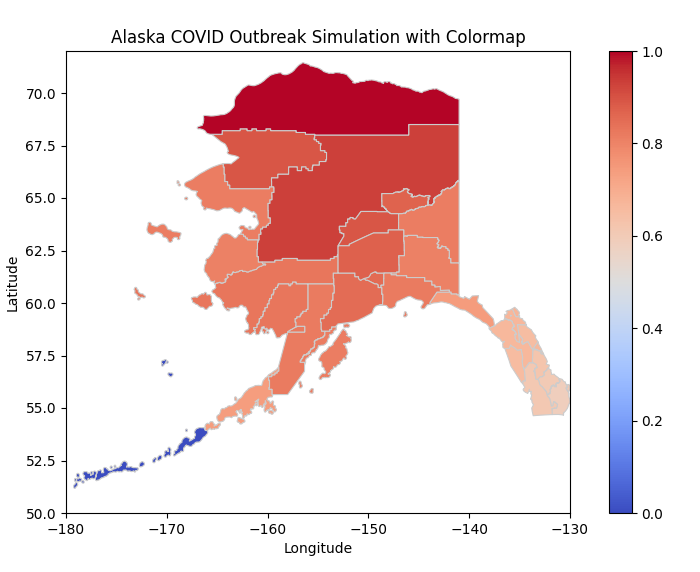
\includegraphics[width=\linewidth]{AlaskaOutbreakExamplev2.png}
  \caption{Sample example of if an outbreak occurred in Alaska starting in North Slope.}
  \Description{Sample example of if an outbreak occurred in Alaska starting in North Slope.}
\end{figure}



\section{Evaluation Methods}
Our group is expecting to measure our success based on our ability to answer the interesting questions set forth here and revised based on our exploration of the data throughout the semester. Objective and subjective evaluation methods will be used for this. As we have seen in the lecture slides, strong association rules are sometimes misleading and we have to use our objective judgment to evaluate the data. Additionally, we will conduct comparative analyses with previous findings, as COVID-19 has been extensively studied. This comparison will allow us to assess the consistency of our results with existing literature and contribute to the broader understanding of the virus's impact.


\section{Tools}
Python Programming language with data science libraries will be used in this project. Python is easy to use and supports wide variety of data science libraries. In addition, Python has a large community which publish tutorials and provides support in online forums.
The following supportive tools will be used in the project. 
\begin{itemize}
\item \textbf{Overleaf} for drafting of our project proposal and presentation(s) to allow for real-time collaboration and updates.
\item \textbf{Git/GitHub} for version control and collaboration.
\item \textbf{Pandas} for manipulating numerical tables and time series as it provides high level abstraction and supports a wide variety of data types.
\item \textbf{NumPy} for simple multi-dimensional arrays and matrices mathematical operations.
\item For data visualization we are considering: \textbf{Tableau, Plotly} and \textbf{Matplotlib}. Tableau and Plotly are interactive, easy to share, and provide high level graphics. While, Matplotlib is flexible and open source. 
\item \textbf{Geopandas} A choropleth map can be utilized to provide a geographic visualization of virus trends.

\end{itemize}




\section{Milestones}
Our team is planning to meet every Wednesday at 5 PM for quick collaboration discussion. In addition, having 3 hours collaboration session each Saturday Morning. Suggested milestones are below:

\begin{enumerate}
\item Week 9: Complete project proposal.
\item Week 10: Exploratory data analysis.
\item Week 11: Data analysis part 1: Complete data cleaning, prepossessing, and data integration.
\item Week 12: Complete project part 3: Progress Report Assignment.
\item Week 13: Data analysis part 2: Apply data mining techniques 1.
\item Week 14: Data analysis part 3: Apply data mining techniques 2.
\item Week 15: Data analysis part 4: Data visualization, report writing, and presentation recording.  
\end{enumerate}


%%
%% The next two lines define the bibliography style to be used, and
%% the bibliography file.
\bibliographystyle{ACM-Reference-Format}
\bibliography{sample-base}


\end{document}
\endinput
%%
%% End of file `sample-sigconf.tex'.
